\documentclass[type=bsc,accentcolor=tud9a,colorback,11pt,paper=a4report]{tudthesis}

\usepackage[utf8]{inputenc}
\usepackage[english]{babel}
\usepackage{listings}
\usepackage{color}
\usepackage{graphicx}
\usepackage{tikz}
\usetikzlibrary{shapes, shadows, arrows, decorations.pathreplacing}

\usepackage{parskip}
\setlength{\parindent}{15pt}
%\usepackage[none]{hyphenat}
\linespread{1.2}
\definecolor{mygreen}{rgb}{0,0.6,0}
\definecolor{mygray}{rgb}{0.5,0.5,0.5}
\definecolor{mymauve}{rgb}{0.58,0,0.82}

\thesistitle{Switching the TCP Congestion Control at Runtime}{}
\department{Fachbereich Informatik}
\group{Databases and Distributed Systems}
\referee{Alexander Frömmgen}{}
\author{Othmane Achoual}

\begin{document}
\makethesistitle
\affidavit{O. Achoual}
\begin{abstract}

	Different applications may have varying needs in bandwidth throughout 
	their execution. Users may also feel the need to prioritize
	certain applcations for some period of time, for example they may want 
	to reduce the bandwidth used by a file download for a few
	minutes in order to have optimal quality on a video they want to watch.

	There is no way to tell the server to reduce its sending
	rate. In this thesis we explore a different approach which is limiting 
	bandwidth of an application through having different flows
	assume different congestion control algorithms, the logic here is that 
	the applications with high priority will assume aggresive
	algorithms whereas those with less priority will assume algorithms that 
	are more conservative.
	
	In linux congestion control
	algorithms can be set on the fly on a per socket basis but only on the 
	local host which is not very helpful for our considered scenario.
	So we take the approach
	of extending TCP with an option that will request from the server to 
	switch the algorithm on the particular socket on which the
	connection is established. To that end we will need to modify the linux 
	kernel on both the host and the server so that this
	new option is recognized by both hosts also a protocol will need to be 
	devised so that the semantics of the option are clear.

	This approach is simulated on a very basic topology but which 
	corresponds to very concrete usage scenarios. We use mininet
	for the simulation due to its capability of emulating complex networks 
	on very simple hardware like a notebook.
\end{abstract}
\tableofcontents
\listoffigures
\lstlistoflistings

\chapter{Introduction}
	In a network bandwidth is a precious resource because it is not 
	extensible. Many times a user may want to allocate more network 
	bandwidth to some application at the expense of limiting it for some 
	other one(s). One way to achieve this would simply be shutting 
	down the application
	that we don't care about, this solution however is a little too radical 
	and we 
	may want the application to stay active, for example we do not want to
	interrupt a file download since we would need to restart the whole 
	process later.

	To influence the amount of bandwidth allocated to each flow on a link
	the idea is to leverage the congestion control mechanism offered to us
	by the transportt layer protocol TCP. This mechanism is normally there
	to ensure that the different flows get a fair amount of bandwidth while
	at the same time ensuring a near optimal network utilization.

	Congestion control algorithms vary on different key aspects in their
	operation like how
	congestion is detected and what steps are taken in reaction to it.
	For example some 
	algorithms will consider increasing Round Trip Times to signify 
	the onset of a
	congestion and react promptly while others will only switch to congestion
	avoidance after a number of packets have been lost. 
	Similarily some algorithms
	will reset their congestion window to the minimum after congestion
	detection while others will restart with some higher value for the 
	congestion window. Those different
	strategies may lead us to consider that some algorithms are more or 
	less conservative or aggressive than others.

	Switching congestion control can only occur on the local host either 
	globally through the procfs filesystem or on a socket basis through
	socket options. This
	doesn't suit our usage scenario since we expect the flow of data to be
	larger from the remote host to the local one and not the opposite. 
	To remedy to this limitation we take 
	the approach of leveraging the opportunity that is given to us by the
	TCP options mechanism. This is achieved by adding
	a new TCP option to the already existing standard ones 
	that when sent to the server  should advise him
	to trigger a switch in congestion control on his side.

	For this it was necessary to explore the kernel source code in order to
	determine where
	the congestion control logic is implemented, what data structures it
	relies on and how it interacts with the rest of the TCP protocol
	implementation. We also needed to find out how TCP options are written 
	passed and
	parsed to support our approach.

	Once the kernel is modified and adapted to support the new TCP option
	we would need to do some testing to find out if the intuition that
	we had about the interaction of aggresive and conservative congestion
	avoidance algorithms was accurate and if in fact we see the allocation
	in bandwidth vary in the way that we expected, namely that the 
	prioritized applications will get more than their fair share through
	this mechanism.

	To carry this evaluation we make use of mininet a network emulation framework that 
	exhibits the benefit of being very lightweight and enables us to
	emulate very complex topologies on very simple hardware. We
	consider a simple topology that exhibits the scenario we are
	interested in. It consists of two servers and a client on
	which two applications are running effectively sharing the
	same network link.
	\section{Structure of the thesis}
Structure of the thesis goes here.
\chapter{The Transmission Control Protocol (TCP)}
	\section{TCP's role in the network stack}
Reliable communication channel on top of unreliable network. In the OSI model the transport layer is responsible for providing a the facilities that enable the 
transmission of data between two processed running on two end hosts on a 
network. 

The protocols that
are part of that layer can fall into one of two categories, connection oriented 
and non connection oriented. A non connection oriented protocol simply tries its best to get the bytes from one host to another over the network
in doing so it doesn't give any guarantee on delivery, ordering and so on. 
The most prominent representative of this category is UDP. 

Naturally connection 
oriented protocols as their name imply serve the purpose of providing a reliable
communication channel between two hosts. This means that it offers a number of 
guarantees to its users from which order of delivery, acknowledgements, 
retransmission and so on. TCP also support other facilities such as Flow control
and Congestion Control. 

Flow control deals with preventing a fast transmitter 
from flooding a slow receiver, to this end both parties advertise to each other 
what is referred to as a window, this window represents the buffer space 
available at the host for dealing with data incoming from that particular TCP 
connection, as the buffer space is filled and consumed the advertised window 
size increases and decreases, this mechanism is referred to as a sliding window.

The Other responsibility that falls on TCP is that of congestion control, while 
the term may point at thinking that this is similar to flow control, it must be 
understood that this deals with the case in which a host sends much more data
than the network not the host can handle, suppose following two hosts with a 
10 Mbits bw, if the host sends at 100 then the network is congested.

\section{Phases of a TCP connection}
Describe 3-way Handshake ...
	\begin{figure}[h]
		\caption{The 3 way Handshake}
		\label{fig:handshake3w}
		\centering
		\includegraphics[width=0.5\textwidth]{hpbn_0201}
	\end{figure}
	\section{The TCP Header}
Introduce the different fields SYN, SYNACK, ACK, FIN, wnd, options.\\
Explain the role of the options as mean to expand TCP and therefore why they 
are suited for our goal.

The tcp functionality is made possible through the TCP Header that is appended 
to each outgoing segment and then passed to the network layer.
It contains all the information that the peer needs to manage most of the 
various tcp operations mentioned previously. The header is represented
by figure \ref{fig:tcpheader}.

	\begin{figure}[h]
		\caption{The TCP Header}
		\label{fig:tcpheader}
		\centering
		\includegraphics[width=0.5\textwidth]{tcpheader}
	\end{figure}
Now we look at the most important fields:

The Options field was designed as a mean to extend the capabilities of the TCP
protocol beyond what its designers originally envisioned to be the essential set
of features. This design was largely influenced by the conditions encountered in
most networks at the time.

For example the
field for the sliding window limits it to a certain size, but thanks to the
wndscale option this window can be multiplied by this factor to lift the
limitation. Likewise they make possible selective acks, so we only resend the
packets that have been lost and not the ones that arrived but out of order.

For this reasons it was natural to rely on TCP options to implement our
extension of the TCP protocol.
	\section{Congestion control mechanisms}
Introduce concepts such as AIMD, Slow start, CWND, Fast recovery, Available 
Algorithms: BIC, CUBIC, VEGAS, RENO, ...
\begin{itemize}
\item Cubic: Cubic is good for networks with high bandwidth.
\item Reno: Reno is statndard TCP implementation with AIMD, Fast recovery,
	suffers from hign RTTs on hign bandwidth network.
\item Vegas: Reno but reacts to Delay rather than loss which makes it weaker.
\end{itemize}
Congestion control is implemented in classic TCP following the AIMD principle 
wich 
stands for Additive Increase Multiplicative Decrease
It has been shown both empirically and with a geometric argument 
\cite{tannenbaum} that 
this mechanism is the only one that converges to a bandwidth allocation that is
both fair and almost optimal for all flows that share some link.
\\Why some algorithms may be more aggressive than others ?\\
A congestion control algorithm can be characterized by how it detects congestion
and how it reacts to it. There are algorithms that are Loss based, meaning
they only interpret packet loss as congestion, while other algorithms are
delay based, meaning they consider increasing RTT values to signal a congestion.

Already we can guess that a Delay based algorithm will enter congestion avoidance
well before a Loss based one which puts him at a disadvantage. Furthermore some
algorithms will increase their window much faster than others so it is legitimate
to think that those will have higher link occupancy over time.
\chapter{Congestion control and TCP Options implementation in the Linux Kernel}
\section{Pluggable congestion control with Strategy pattern implementation in C}
Inside the linux kernel the congestion control algorithms are swapped for each 
other in what in essence is an application of the famous strategy pattern 
\cite{gamma}. However, since The C programming language is an imperative 
language 
rather than an Object Oriented one, the linux kernel approximates what in some
OO languages like JAVA is called an interface by defining a structure 
consisting of function pointers having the signature of the different methods 
that needs to be implemented by a congestion algorithm. 

These procedures are 
responsible for example for updating the congestion window. Each connection 
oriented socket has one such struct as a member, that way changing congestion
control for a particular socket is simply a matter of assigning a new 
tcp\_congestion\_ops structure to this member.

A new congestion control algorithm can be added simply by defining concrete 
procedures with the same signature and then populating the tcp\_congestion\_ops 
struct with pointers to these implementations, then all that is left to do is 
registering this struct with the kernel. 
The different congestion control algorithms can either be compiled inside the
kernel image or built as separate modules. In the latter case the registration 
will happen when the specific module is loaded, either at bootup for the default
algorithm or after that if the request is through sysctl or socketoption. 
In both cases if the congestion algorithm is built as a module the kernel will 
look for it following a predefined naming convention load it and the init method
of the module will take care of the registration.

		%\lstinputlisting[language=c]{piapprox.c}
		\lstset{ %
		backgroundcolor=\color{white},   % choose the background color; you must add \usepackage{color} or \usepackage{xcolor}
		basicstyle=\footnotesize,        % the size of the fonts that are used for the code
		breakatwhitespace=false,         % sets if automatic breaks should only happen at whitespace
		breaklines=true,                 % sets automatic line breaking
		captionpos=b,                    % sets the caption-position to bottom
		commentstyle=\color{mygreen},    % comment style
		morecomment=[s]{/*}{*/},
		morecomment=[l]{/*}{*/},
		deletekeywords={...},            % if you want to delete keywords from the given language
		escapeinside={\%*}{*)},          % if you want to add LaTeX within your code
		extendedchars=true,              % lets you use non-ASCII characters; for 8-bits encodings only, does not work with UTF-8
		frame=single,	                   % adds a frame around the code
		keepspaces=true,                 % keeps spaces in text, useful for keeping indentation of code (possibly needs columns=flexible)
		keywordstyle=\color{blue},       % keyword style
		language=C,                 % the language of the code
		otherkeywords={...},           % if you want to add more keywords to the set
		numbers=left,                    % where to put the line-numbers; possible values are (none, left, right)
		numbersep=5pt,                   % how far the line-numbers are from the code
		numberstyle=\tiny\color{mygray}, % the style that is used for the line-numbers
		rulecolor=\color{black},         % if not set, the frame-color may be changed on line-breaks within not-black text (e.g. comments (green here))
		showspaces=false,                % show spaces everywhere adding particular underscores; it overrides 'showstringspaces'
		showstringspaces=false,          % underline spaces within strings only
		showtabs=false,                  % show tabs within strings adding particular underscores
		stepnumber=1,                    % the step between two line-numbers. If it's 1, each line will be numbered
		stringstyle=\color{mymauve},     % string literal style
		tabsize=2,	                   % sets default tabsize to 2 spaces
		title={tcp\_congestion\_ops structure}                  % show the filename of files included with \lstinputlisting; also try caption instead of title
		}
		\lstinputlisting[label=tcpcongestionops, caption=the tcp\_congestion\_ops struct]{congestion_ops.c}

	\section{The tcp\_sock structure}
Inheritance like mechanism allow it to extend the functionality of more general socket structures, keeps track of received options and other TCP related parameters.

Fundamental to the implementation of the TCP protocol in the linux kernel is 
the tcp\_sock structure. this struct defined in \emph{include/linux/tcp.h} is 
responsible for tracking all the relevant information that allows a TCP 
connection to operate properly. 

Like mentioned previously native Object Oriented Programming constructs 
are not present in C but still the linux kernel emulates inheritance for 
tcp\_sock from the connection\_sock struct by having an instance of it as the 
first member of the tcp\_sock struct that way and thanks to the data 
organization of C 
a tcp\_sock can be cast to connection\_sock as needed and connection oriented 
sockets for protocols other than TCP can be built on top of connection\_sock
retaining all of its functionality.

This structure keeps track of information such as MSS, estimated RTT and many
more and is updated during the whole lifetime of the connection to reflect the 
current values for these parameters, some of which are affected by the received 
options. For this reason this will be the structure where we will mark if a 
congestion needs to be requested on the next sent packet(s) or if a confirmation
of a successful or unsuccessful switch needs to be sent.
	\section{The tcphdr structure}
where is it defined, Models the TCP Header previously discussed 
(Don't know if this deserves its own section)
\chapter{Modifying the Linux Kernel to enable congestion control switching at runtime}
	\section{Format of the new Option and how it works}
Still not finialized, questions remain, should we acknowledge, retransmit, for how many times ?

In order not to clutter the header with our new option, we decided to pack it in 
4 Bytes, meaning we are occupying the least amount of space for a TCP
option since all options should be aligned on 4 Byte boundaries. 
The option follows the format of the other standard TCP options which 
makes it possible to process it by the already existing facilities in the linux 
kernel.

The Option consists of the usual option code and option length fields, 
the body of the 
option consists of 3 flags req, conf and neg. plus fields for the enumerated 
congestion algorithms that occupy 5 bits so we support up to 31 algorithms one 
field is for 
requesting and the other for confirming, this makes it possible to request and 
confirm on the same packet. The body of the new option is illustrated in Figure
\ref{fig:option}.

\begin{figure}[h]
\centering
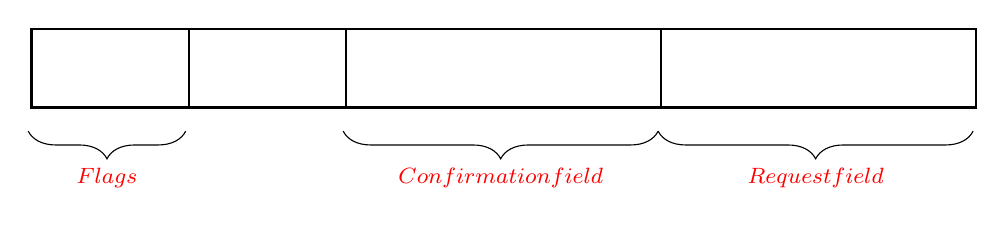
\begin{tikzpicture}
	\draw[thick] (0,0) rectangle +(2, 1);
\draw [decorate,decoration={brace,amplitude=10pt,mirror},xshift=-4pt,yshift=0pt]
	(0.1,-0.3) -- +(2,0) node [red,midway,xshift=0.0cm, yshift=-0.6cm] 
	{\footnotesize $Flags$};
	\draw[thick] (2,0) rectangle +(2, 1);
	\draw[thick] (4,0) rectangle +(4, 1);
\draw [decorate,decoration={brace,amplitude=10pt,mirror},xshift=-4pt,yshift=0pt]
	(4.1,-0.3) -- +(4,0) node [red,midway,xshift=0.0cm, yshift=-0.6cm] 
	{\footnotesize $Confirmation field$};
	\draw[thick] (8,0) rectangle +(4, 1);
\draw [decorate,decoration={brace,amplitude=10pt,mirror},xshift=-4pt,yshift=0pt]
	(8.1,-0.3) -- +(4,0) node [red,midway,xshift=0.0cm, yshift=-0.6cm] 
	{\footnotesize $Request field$};

\end{tikzpicture}
\caption{tcp congestion request option}
\label{fig:option}
\end{figure}

The protocol is a very simple one, once a congestion control is requested by the
application, each transmitted packet will be tagged with an option with the 
request bit set and the value of the enum in the request field until we
receive either a positive or negative confirmation in which case we
cease sending the option. On the server side once we receive the option
we try to set the congestion control accordingly and etither send an
option confirming or negating the success of the operation. This works
since setting congestion control is idempotent so setting an existing
congestion control has no bad side effects. The mechanism can be made
cleaner by waiting for a certain amount like an RTT before retransmitting 
a request or a confirmation, but for our purpose this is good enough.
	\section{Modifying the files}
		Describe the modifications to each of the files
		/include/uapi/linux/tcp.h /include/linux/tcp.h /net/ipv4/tcp.c ...
\chapter{Evaluating the Results}
	\section{Tools of the trade}
	Mininet, Gnuplot, wireshark ? (Don't know if we need to use it)\\
	\section{Considered Scenario(s)}
	Topology, Number of servers, Number of clients, Link Capacity/Delay\\
	How many runs ? Simulation duration, Statistical quantities(average, variance, ...)
	\section{Actual Results Evaluation}
	What algorithms perform better against which others and in which scenario ?\\
	Based on this when would it make sense to switch ?
\chapter{Conclusion}
	Wrap up of key results and remarks.
\begin{thebibliography}{1}
	\bibitem{tannenbaum} Andrew Tannenbaum, \emph{Computer Networks}.
	\bibitem{gamma} Erich Gamma, John Vlissides, Ralph Johnson and Richard Helm, \emph{Design Patterns Elements of Reusable Object-Oriented Software}.
\end{thebibliography}
\end{document}
